\tikzset{every picture/.style={line width=0.75pt}} %set default line width to 0.75pt        
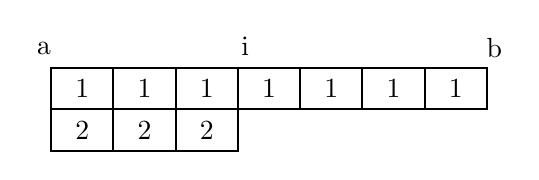
\begin{tikzpicture}[x=0.75pt,y=0.75pt,yscale=-1,xscale=1]
%uncomment if require: \path (0,74.33332824707031); %set diagram left start at 0, and has height of 74.33332824707031

%Shape: Rectangle [id:dp6287463531133186] 
\draw   (20,20) -- (50,20) -- (50,40) -- (20,40) -- cycle ;
%Shape: Rectangle [id:dp6712332802681875] 
\draw   (50,20) -- (80,20) -- (80,40) -- (50,40) -- cycle ;
%Shape: Rectangle [id:dp8581103754160746] 
\draw   (80,20) -- (110,20) -- (110,40) -- (80,40) -- cycle ;
%Shape: Rectangle [id:dp6750047382984976] 
\draw   (110,20) -- (140,20) -- (140,40) -- (110,40) -- cycle ;
%Shape: Rectangle [id:dp7403561919997843] 
\draw   (140,20) -- (170,20) -- (170,40) -- (140,40) -- cycle ;
%Shape: Rectangle [id:dp644418423147074] 
\draw   (170,20) -- (200,20) -- (200,40) -- (170,40) -- cycle ;
%Shape: Rectangle [id:dp6636672838250548] 
\draw   (200,20) -- (230,20) -- (230,40) -- (200,40) -- cycle ;
%Shape: Rectangle [id:dp2893216606013862] 
\draw   (80,40) -- (110,40) -- (110,60) -- (80,60) -- cycle ;
%Shape: Rectangle [id:dp4354422116955303] 
\draw   (20,40) -- (50,40) -- (50,60) -- (20,60) -- cycle ;
%Shape: Rectangle [id:dp9120747157270248] 
\draw   (50,40) -- (80,40) -- (80,60) -- (50,60) -- cycle ;

% Text Node
\draw (35,30) node   [align=left] {\cancel{1}};
% Text Node
\draw (65,30) node   [align=left] {\cancel{1}};
% Text Node
\draw (95,30) node   [align=left] {\cancel{1}};
% Text Node
\draw (155,30) node   [align=left] {1};
% Text Node
\draw (125,30) node   [align=left] {1};
% Text Node
\draw (185,30) node   [align=left] {1};
% Text Node
\draw (215,30) node   [align=left] {1};
% Text Node
\draw (35,50) node   [align=left] {2};
% Text Node
\draw (65,50) node   [align=left] {2};
% Text Node
\draw (95,50) node   [align=left] {2};
% Text Node
\draw (16.5,10.5) node   [align=left] {a};
% Text Node
\draw (233.5,10.5) node   [align=left] {b};
% Text Node
\draw (113.5,9.5) node   [align=left] {i};


\end{tikzpicture}
